\section{Early Design Mockups}
\label{app:early-design-mockups}

The following figures collect the early visual references that informed the design choices described in the solution section.

\begin{figure}[H]
  \centering
  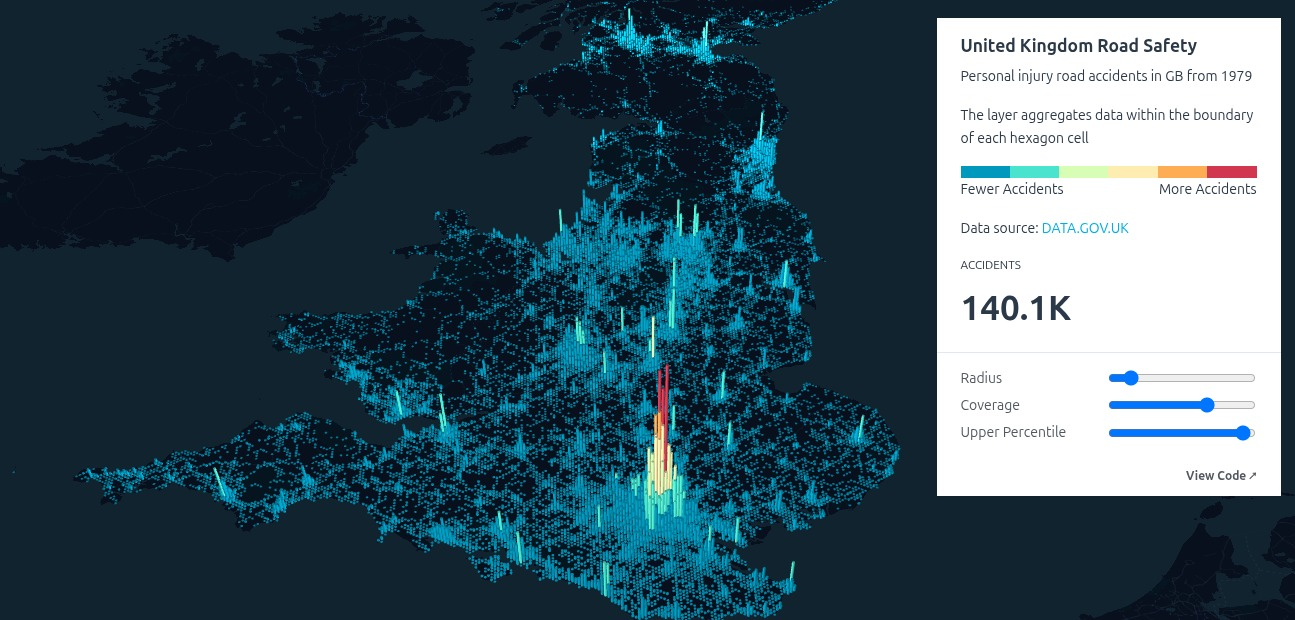
\includegraphics[width=0.7\textwidth]{../media/proposal/heatmap.jpeg}
  \caption{Example of a map-based density layer. In our dashboard, a similar encoding could represent station-level or area-level demand, using height and color intensity to make spatial hotspots immediately visible.}
  \label{fig:mockup-heatmap}
\end{figure}

\begin{figure}[H]
  \centering
  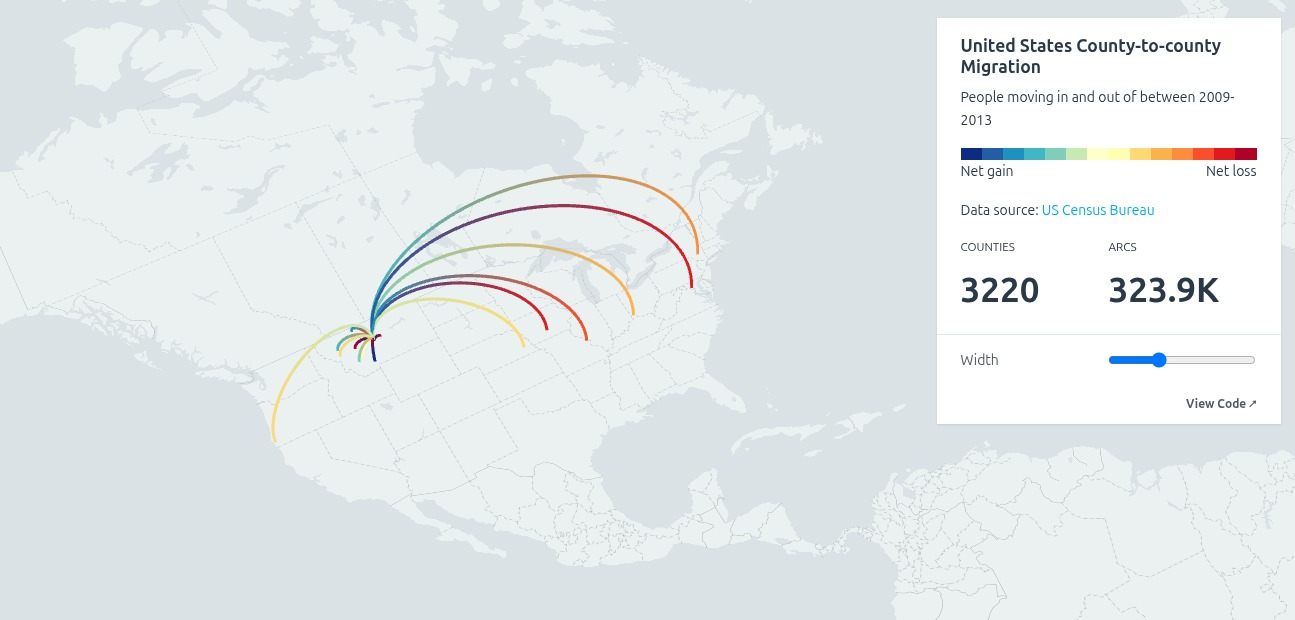
\includegraphics[width=0.7\textwidth]{../media/proposal/trip-layer.jpeg}
  \caption{Example of an origin-destination flow layer. For \texttt{Citi Bike}, this approach could be adapted to show the strongest station-to-station movements, commute corridors, or directional differences between selected areas.}
  \label{fig:mockup-trip-layer}
\end{figure}

\begin{figure}[H]
  \centering
  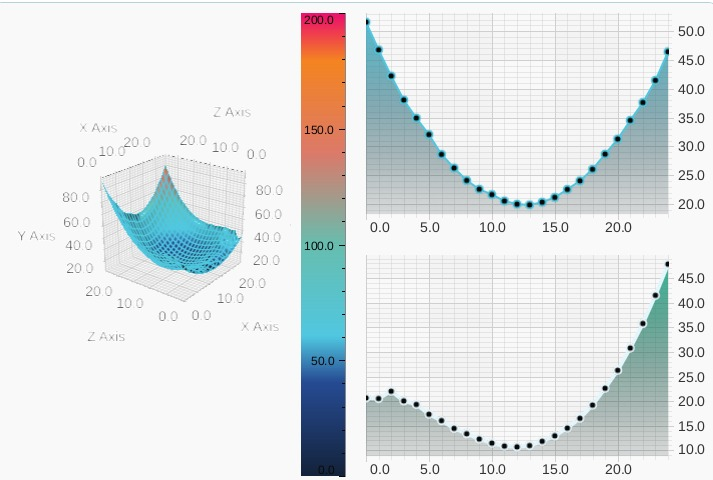
\includegraphics[width=0.6\textwidth]{../media/proposal/surface-graph.jpeg}
  \caption{Example of a temporal comparison view. The combination of a surface plot and aligned line charts suggests how we could compare ridership intensity across hours, days, or seasons while still allowing detailed inspection of selected time slices.}
  \label{fig:mockup-surface-graph}
\end{figure}

\begin{figure}[H]
  \centering
  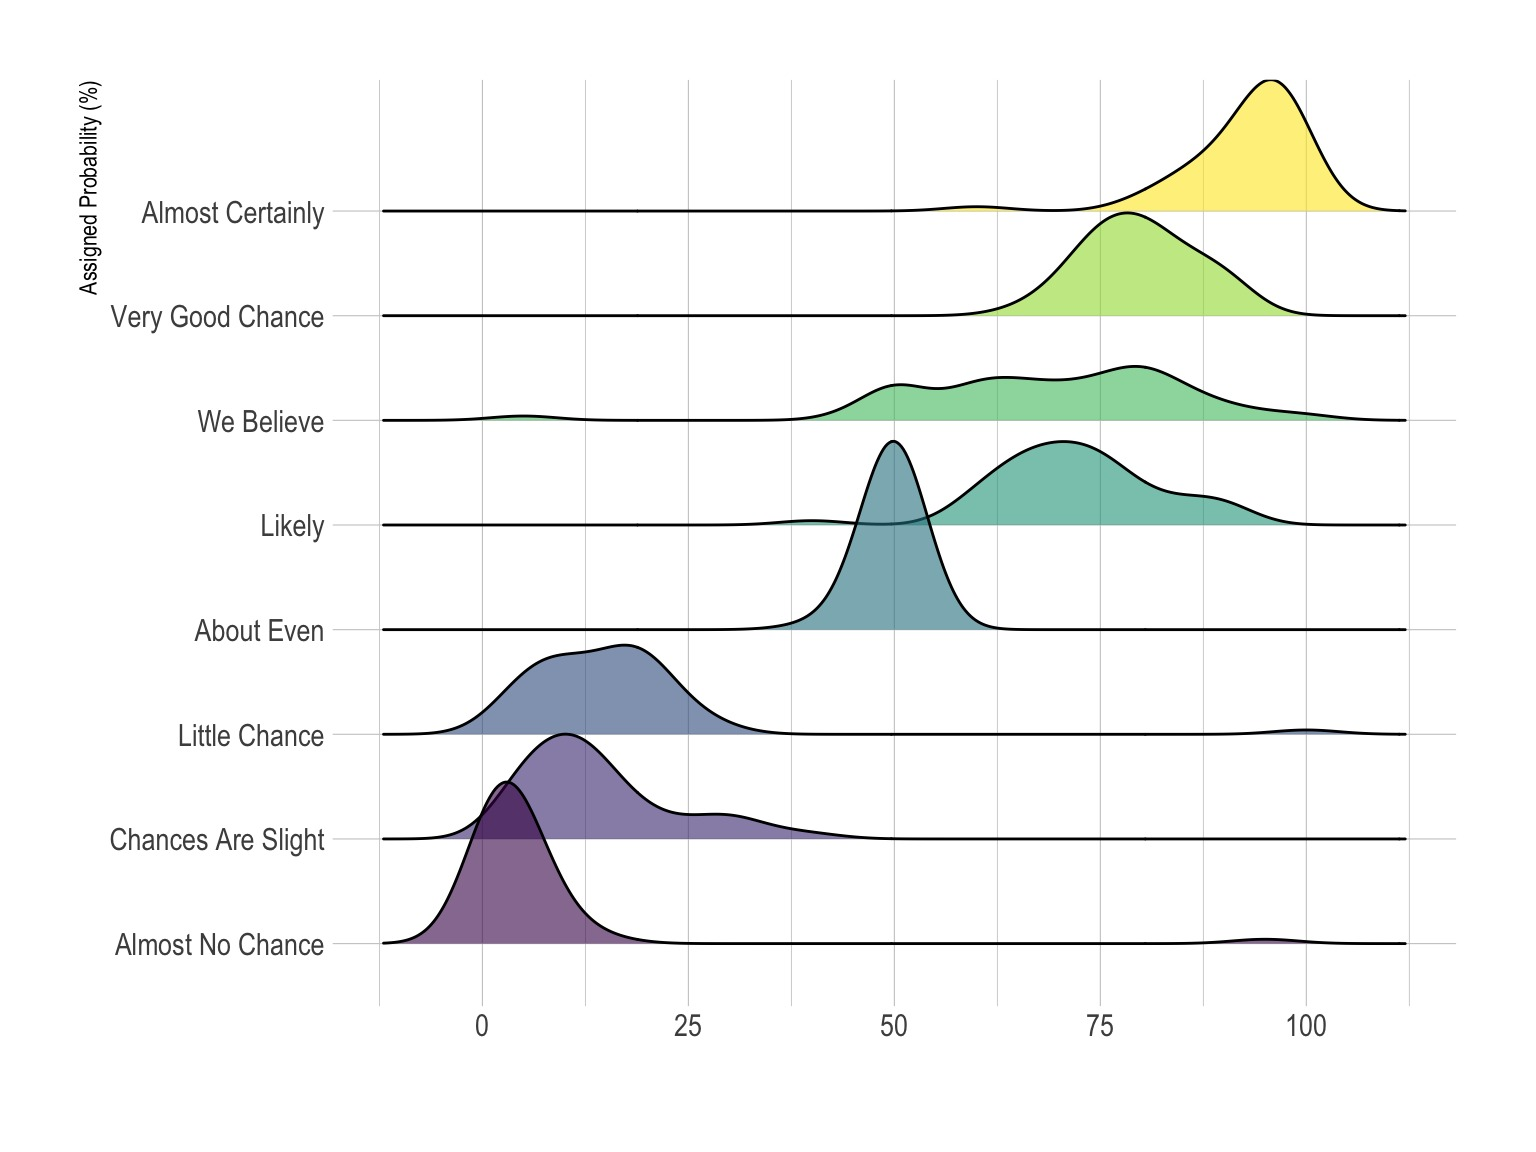
\includegraphics[width=0.7\textwidth]{../media/proposal/ridge-graph.jpeg}
  \caption{Example of a ridge plot for comparing distributions across ordered categories. In our case, this kind of view could support comparisons of ride volumes or trip durations under different weather conditions, such as temperature ranges, rainfall levels, or wind intensity.}
  \label{fig:mockup-ridge-graph}
\end{figure}
